%------------------------------------------------------------------------------
% CV in Latex
% Author : Charles Rambo
% Based off of: https://github.com/sb2nov/resume and Jake's Resume on Overleaf
% Most recently updated version may be found at https://github.com/fizixmastr 
% License : MIT
%------------------------------------------------------------------------------

\documentclass[a4paper,11pt]{ctexart}
%\documentclass[letterpaper,11pt]{article} %For use in US
\usepackage{latexsym}
\usepackage[empty]{fullpage}
\usepackage{titlesec}
\usepackage{marvosym}
\usepackage[usenames,dvipsnames]{color}
\usepackage{verbatim}
\usepackage{enumitem}
\usepackage[hidelinks]{hyperref}
\usepackage[english]{babel}
\usepackage{tabularx}
\usepackage{tikz}
%\input{glyphtounicode}

\usepackage{makecell}

\begin{comment}
I am by no means a professional when it comes to the CV's/resumes, I have
received various trainings on how to write a CV and resume from my high 
school, as well as the Austin College and University of Eastern Finland's
career counseling departments. As I intend to share my CV as a template, I 
feel that it is my responsibility to provide explanations of my work.
\end{comment}


%-----FONT OPTIONS-------------------------------------------------------------
\begin{comment}
The font of the document will impact not just how readable it is, but how it is
perceived. In the "The Craft of Scientific Writing" by Michael Alley, shares a
common fonts for publication as well as their use. I have chosen to use
Palatino for its legibility, some others are given below. There is far too much
about typography to discus here. Note: serif fonts have short projecting
strokes, sans-serif fonts are sans (without) these strokes.
\end{comment}


% serif
%\usepackage{palatino}
%\usepackage{times} %This is the default as well
% \usepackage{charter}

% sans-serif
% \usepackage{helvet}
% \usepackage[sfdefault]{noto-sans}
% \usepackage[default]{sourcesanspro}

%-----PAGE SETUP---------------------------------------------------------------

% Adjust margins
\addtolength{\oddsidemargin}{-1cm}
\addtolength{\evensidemargin}{-1cm}
\addtolength{\textwidth}{2cm}
\addtolength{\topmargin}{-1cm}
\addtolength{\textheight}{2cm}

% Margins for US Letter size
%\addtolength{\oddsidemargin}{-0.5in}
%\addtolength{\evensidemargin}{-0.5in}
%\addtolength{\textwidth}{1in}
%\addtolength{\topmargin}{-.5in}
%\addtolength{\textheight}{1.0in}

\urlstyle{same}

\raggedbottom
\raggedright
\setlength{\tabcolsep}{0cm}

% Sections formatting
\titleformat{\section}{
	\vspace{-4pt}\scshape\raggedright\large
}{}{0em}{}[\color{black}\titlerule \vspace{-5pt}]

% Ensure that .pdf is machine readable/ATS parsable
%\pdfgentounicode=1

%-----CUSTOM COMMANDS FOR FORMATTING SECTIONS----------------------------------
\newcommand{\CVItem}[1]{
	\item\small{
		{#1 \vspace{-2pt}}
	}
}

\newcommand{\CVSubheading}[4]{
	\vspace{-2pt}\item
	\begin{tabular*}{0.97\textwidth}[t]{l@{\extracolsep{\fill}}r}
		\textbf{#1} & #2 \\
		\small#3 & \small #4 \\
	\end{tabular*}\vspace{-7pt}
}

\newcommand{\CVSubSubheading}[2]{
	\item
	\begin{tabular*}{0.97\textwidth}{l@{\extracolsep{\fill}}r}
		\text{\small#1} & \text{\small #2} \\
	\end{tabular*}\vspace{-7pt}
}

\newcommand{\CVSubItem}[1]{\CVItem{#1}\vspace{-4pt}}

\renewcommand\labelitemii{$\vcenter{\hbox{\tiny$\bullet$}}$}

\newcommand{\CVSubHeadingListStart}{\begin{itemize}[leftmargin=0.5cm, label={}]}
	% \newcommand{\resumeSubHeadingListStart}{\begin{itemize}[leftmargin=0.15in, label={}]} % Uncomment for US
	\newcommand{\CVSubHeadingListEnd}{\end{itemize}}
\newcommand{\CVItemListStart}{\begin{itemize}}
	\newcommand{\CVItemListEnd}{\end{itemize}\vspace{-5pt}}

%------------------------------------------------------------------------------
% CV STARTS HERE  %
%------------------------------------------------------------------------------
\begin{document}
	
	%-----HEADING------------------------------------------------------------------
	\begin{comment}
	In Europe it is common to include a picture of ones self in the CV. Select
	which heading appropriate for the document you are creating.
	\end{comment}
	
	\begin{minipage}[c]{0.05\textwidth}
		\-\
	\end{minipage}
	\begin{minipage}[c]{0.21\textwidth}
		\begin{tikzpicture}
			\clip (0,0) circle (1.5cm);
			\node at (0,-0.4) {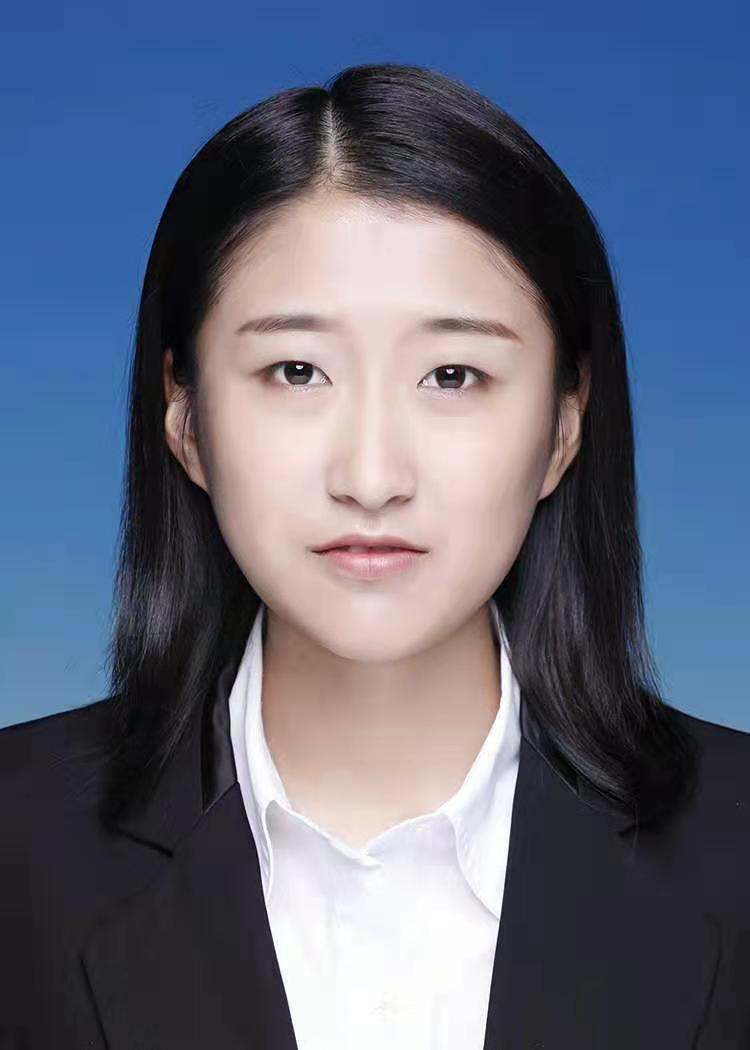
\includegraphics[width = 3cm]{portrait}}; 
			% if necessary the picture may be moved by changing the at (coordinates)
			% width defines the 'zoom' of the picture
		\end{tikzpicture}
		\hfill\vline\hfill
	\end{minipage}
	\begin{minipage}[c]{0.4\textwidth}
		\textbf{\Huge \scshape{吴航}} \\ \vspace{1pt} 
		% \scshape sets small capital letters, remove if desired
		\small{(+86) 159-3536-6489} \\
		\small{邮箱: \href{mailto:wuhang@xs.ustb.edu.cn}{\underline{wuhang@xs.ustb.edu.cn}}}\\
		\small{期望职位:测试开发实习生} \\
		\small{期望地点:北京} \\
	\end{minipage}
	
	% Without picture
	%\begin{center}
	%    \textbf{\Huge \scshape Charles Rambo} \\ \vspace{1pt} %\scshape sets small capital letters, remove if desired
	%    \small +1 123-456-7890 $|$ 
	%    \href{mailto:you@provider.com}{\underline{you@provider.com}} $|$\\
	%    % Be sure to use a professional *personal* email address
	%    \href{https://linkedin.com/in/your-name-here}{\underline{linkedin.com/in/charles-rambo}} $|$
	%    % you should adjust you linked in profile name to be professional and recognizable
	%    \href{https://github.com/fizixmastr}{\underline{github.com/fizixmastr}}
	%\end{center}
	
	
	
	\begin{comment}
	This CV was written for specifically for positions I was applying for in
	academia, and then modified to be a template.
	
	A standard CV is about two pages long where as a resume in the US is one page.
	sections can be added and removed here with this in mind. In my experience, 
	education, and applicable work experience and skills are the most import things
	to include on a resume. For a CV the Europass CV suggests the categories: Work
	Experience, Education and Training, Language Skills, Digital Skills,
	Communication and Interpersonal Skills, Conferences and Seminars, Creative Works
	Driver's License, Hobbies and Interests, Honors and Awards, Management and
	Leadership Skills, Networks and Memberships, Organizational Skills, Projects,
	Publications, Recommendations, Social and Political Activities, Volunteering.
	
	Your goal is to convey a who, what , when, where, why for every item you share. 
	The who is obviously you, but I believe the rest should be done in that order.
	For example below. An employer cares most about the degree held and typically 
	less about the institution or where it is located (This is still good 
	information though). Whatever order you choose be consistent throughout.
	\end{comment}
	
	%-----EDUCATION----------------------------------------------------------------
	\section{教育经历}
	\CVSubHeadingListStart
	%    \CVSubheading % Example
	%      {Degree Achieved}{Years of Study}
	%      {Institution of Study}{Where it is located}
	\CVSubheading
	{{工学硕士在读 $|$ \emph{\small{计算机科学与技术}}}}{2019.09 -- 2022.06}
	{北京科技大学 -- 计算机与通信工程学院}{北京市海淀区}
	\CVSubheading
	{{工学学士 $|$ \emph{\small{计算机科学与技术}}}}{2015.09 -- 2019.06}
	{中华女子学院 -- 计算机与通信工程学院}{北京市朝阳区}
	\CVSubHeadingListEnd
	
	%-----PROJECTS AND RESEARCH----------------------------------------------------
	\begin{comment}
	Ideally the title of the work should speak for what it is. However if you feel
	like you should explain more about why the project is applicable to this job,
	use item list as is shown in the work experience section.
	\end{comment}
	
	\section{项目经历}
	\CVSubHeadingListStart
	\CVSubheading
	{{趣味强化学习实验平台}  $|$ \emph{\small{Python}}}{2020.03 -- 2020.05}
	{以空战小游戏为背景,开展不稳定环境集群任务协同实验}{}
	\CVItemListStart
	\CVItem{不同角色Agent协同作战,验证多Agent协同框架}
	\CVItem{采用黑板模式进行Agent之间的通信}
	\CVItemListEnd
	\CVSubheading
	{{会议管理系统}  $|$ \emph{\small{JS/Java/Android/MySQL}}}{2018.08 - 2018.09}
	{\makecell[l]{\hspace{2em}2018年(第6届)中国大学生计算机设计大赛软件服务外包竞赛(移动终端应用)。\\
			该管理系统是会议掌管 APP 的后台支撑,提供对会议基本信息进行维护的功能,以及\\
			对人员权限的分配功能。
	}}{}
	\CVItemListStart
	\CVItem{采用相对布局设计UI原型,并对不同大小和分辨率的屏幕进行适配}
	\CVItem{采用线程监听机制进行客户端与服务器端数据传输}
	\CVItemListEnd
	\CVSubheading
	{{共享单车Web管理系统}  $|$ \emph{\small{SSM框架}}}{2018.06 - 2018.08}
	{大三暑期实践,由Oracle公司讲师主讲,主要负责Java后端开发与程序测试}{}
	\CVItemListStart
	\CVItem{采用Spring MVC框架实现单车管理、故障管理和报表统计功能}
	\CVItem{采用Postman工具进行接口自动化测试}
	\CVItemListEnd
	%\CVSubheading
	%{聊天匹配软件$|$ \emph{\small{Android}}}{Fall 2019}
	%{软件外包}{}
	%\CVSubheading
	%{{} $|$ 
	%{}{}
	
	%\CVSubheading
	%{{} \emph{\small{}}}{ 2018}
	%{}{}
	\CVSubHeadingListEnd
	
	%-----WORK EXPERIENCE----------------------------------------------------------
	\begin{comment}
	try to briefly explain what you did and why it is relevant to the position you
	are seeking
	\end{comment}
	
	\section{科研经历}
	\CVSubHeadingListStart
	%    \CVSubheading %Example
	%      {What you did}{When you worked there}
	%      {Who you worked for}{Where they are located}
	%      \CVItemListStart
	%        \CVItem{Why it is important to this employer}
	%      \CVItemListEnd
	\CVSubheading
	{不稳定环境集群任务协同架构 $|$ \emph{\small{专利}}}{2019.12 -- 2020.04}
	{\makecell[l]{\hspace{2em}构建基于角色的多智能体协同模型体系,建立多智能体间通用的分布式自适应的协同任务\\
		处理机制。研究基于角色的多智能任务协同消息传递及异常处理机制}}{}
	\CVSubheading
	{面向自组织局部云的多机器人协作环境态势感知 $|$ \emph{\small{中科院横向项目}}}{2020.05 -- 2020.12}
	{\makecell[l]{\hspace{2em}搭建面向云环境的多机器人自组织协同架构,研究云服务技术下的协同框架,支持协同\\
			态势冲突检测和消解以及失效情况下的重组。}}{}
	\CVSubheading
	{\small\textbf{Constrained Gaussian Condensation Filter for Cooperative Target Tracking} }{2020.7 -- 2021.1}
	{\makecell[l]{\hspace{2em}基于时空约束高斯聚合滤波的协同运动追踪,提出一种基于时空约束高斯聚合滤波的多目标\\
			协同追踪算法,完成空间约束优化时序滤波估计的位置信息。(\textbf{SCI论文在投})}}{}
	\CVSubHeadingListEnd
	
	
	%-----CONFERENCES AND PRESENTATIONS--------------------------------------------
	\begin{comment}
	Again the title should have already been enough, but if it is necessary to add
	descriptions maintain the consistency from prior sections
	\end{comment}
	
	%-----HONORS AND AWARDS--------------------------------------------------------
	\section{获奖经历}
	%    \CVSubheading %Example
	%      {What}{When}
	%      {Short Description}{}
	{北京科技大学研究生二等奖学金}\hfill{Fall 2020}\\
	{中华女子学院国家奖学金}\hfill{Fall 2018} \\
	{全国大学生计算机设计大赛全国二等奖}\hfill{Fall 2018} \\
	{全国大学生数学建模竞赛北京赛区二等奖}\hfill{Fall 2017}\\
	%-----TEACHING EXPERIENCE------------------------------------------------------
	\begin{comment}
	Section is here as it applied to my application for positions in academia. 
	Remember to tailor the resume for to the position.
	\end{comment}
	
	%-----SKILLS-------------------------------------------------------------------
	\begin{comment}
	This section is compressed from the various skills sections that Euro CV
	recommends.
	\end{comment}
	
	%------------------------------------------------------------------------------
\end{document}
